\documentclass[12pt,a4paper]{report}


\usepackage{amsmath}
\usepackage[utf8]{inputenc}
\usepackage{amsmath}
%\usepackage{unicode-math}
\usepackage{amsfonts}
\usepackage{amssymb}
\usepackage{calrsfs}
\usepackage[left=2cm,right=2cm,top=2cm,bottom=2cm]{geometry}
\usepackage[mathscr]{euscript}

\usepackage{color}

%%%%%%%%%%for writing large parallel%%%%%%
\usepackage{mathtools}
\DeclarePairedDelimiter\bignorm{\lVert}{\rVert}
%%%%%%%%%%%%%%%%%%%%%%%%%%%%%%%%%%%%%%%%%%

%%%%%%%%Draws Pretty Box%%%%%%%
%%%Use with \bluebox[<top pad>][<bot pad>]{<contents>}
\definecolor{myblue}{rgb}{.8, .8, 1}

\usepackage{empheq}

\newlength\mytemplen
\newsavebox\mytempbox

\makeatletter
\newcommand\bluebox{%
    \@ifnextchar[%]
       {\@bluebox}%
       {\@bluebox[0pt]}}

\def\@bluebox[#1]{%
    \@ifnextchar[%]
       {\@@bluebox[#1]}%
       {\@@bluebox[#1][0pt]}}

\def\@@bluebox[#1][#2]#3{
    \sbox\mytempbox{#3}%
    \mytemplen\ht\mytempbox
    \advance\mytemplen #1\relax
    \ht\mytempbox\mytemplen
    \mytemplen\dp\mytempbox
    \advance\mytemplen #2\relax
    \dp\mytempbox\mytemplen
    \colorbox{myblue}{\hspace{0em}\usebox{\mytempbox}\hspace{0em}}}
%%%%%%%%%%%%%%%%%%%%%%%%%%%%%%%%%%%%%%%%%%%%%

%%%%%%%%%%for writing symbol above an equality
\newcommand\xeq{\stackrel{\mathclap{\normalfont\mbox{d}}}{=}}
%%%%%%%%%%%%%%%%%%%%%%%%%%%%%%%%%%%%%%%%%%%%

%%%for drawing commutative diagrams.%%%%%%
\usepackage{tikz-cd}  
%%%%%%%%%%%%%%%%%%%%%%%%%%%%%%%%%%%%%%%%%%

%%%%%%%%%%for changing margin
\def\changemargin#1#2{\list{}{\rightmargin#2\leftmargin#1}\item[]}
\let\endchangemargin=\endlist 

\newenvironment{proof}
{\begin{changemargin}{1cm}{0.5cm} 
	}%your text here
	{\end{changemargin}
}

\newenvironment{subproof}
{\begin{changemargin}{0.5cm}{0.5cm} 
	}%your text here
	{\end{changemargin}
}
%%%%%%%%%%%%%%%%%%%%%%%%%%%%%

\begin{document}
\newcommand{\thm}{\textbf{Theorem) }}
\newcommand{\thmnum}[1]{\textbf{Theorem #1) }}
\newcommand{\defi}{\textbf{Definition) }}
\newcommand{\definum}[1]{\textbf{Definition #1) }}
\newcommand{\lem}{\textbf{Lemma) }}
\newcommand{\lemnum}[1]{\textbf{Lemma #1) }}
\newcommand{\prop}{\textbf{Proposition)}}
\newcommand{\propnum}[1]{\textbf{Proposition #1) }}
\newcommand{\corr}{\textbf{Corollary) }}
\newcommand{\corrnum}[1]{\textbf{Corollary #1) }}
\newcommand{\pf}{\textbf{proof) }}


\newcommand{\lap}{\triangle} %%Laplacian
\newcommand{\s}{\vspace{10pt}}
\newcommand{\bull}{$\bullet$}
\newcommand{\sta}{$\star$}
\newcommand{\reals}{\mathbb{R}}

\newcommand{\eop}{\hfill  \textsl{(End of proof)} $\square$} %end of proof
\newcommand{\eos}{\hfill  \textsl{(End of statement)} $\square$} %end of proof


\newcommand{\intN}{\mathbb{Z}_N}
\newcommand{\nat}{\mathbb{N}}
\newcommand{\norms}[2]{\bignorm[\big]{#1}_{#2}}
\newcommand{\avg}{\mathbb{E}}
\newcommand{\prob}{\mathbb{P}}
\newcommand{\borel}{\mathscr{B}}
\newcommand{\EE}{\mathscr{E}}
\newcommand{\F}{\mathscr{F}}
\newcommand{\W}{\mathscr{W}}
\newcommand{\cov}{\text{Cov}}
\newcommand{\var}{\text{Var}}
\newcommand{\cha}{1}

\newcommand{\newday}{===============================================================}

\setlength\parindent{0pt}

\chapter*{Advanced Probability}
\s

\newday

(2nd November, Friday)

\section*{Chapter 5. Weak Convergence}

\subsection*{5.1. Definitions}

Let $E$ be a metric space. Whenever we are talking about a metric space, the $\sigma$-algebra is given by the Borel $\sigma$-algebra. Write $C_b(E)$ for the set of bounded continuous functions on $E$.
\begin{itemize}
\item Let $(\mu_n :n\in \mathbb{N})$ be a sequence of probability measures and let $\mu$ be another probability measure on $E$. We say that $\mu_n \rightarrow \mu$ \textbf{weakly} (as $n\rightarrow \infty$) if $\mu_n (f) \rightarrow \mu(f)$ for all $f\in C_b(\reals)$.
\end{itemize}
\s

\thmnum{5.1.1} The following are equivalent.
\begin{itemize}
\item[(a)] $\mu_n \rightarrow \mu$ weakly on $E$
\item[(b)] $\liminf_{n\rightarrow \infty} \mu_n(U) \geq \mu(U)$ for all $U$ open
\item[(c)] $\limsup_{\mu(F)} \leq \mu(F)$ for all $F$ closed.
\item[(d)] $\mu_n(B) \rightarrow \mu(B)$ for all $B \in \borel$ such that $\mu(\partial B)=0$.(Boundary is the set of limit points of $B$ that are not contained in $B$.)
\end{itemize}
\begin{proof}
\pf Exercise.
\end{proof}
\s

For an example, consider a sequence $(x_n)_n \subset \reals$ such that $x_n \rightarrow 0$ as $n\rightarrow \infty$. We want to have $\delta_{x_n} \rightarrow \delta_0$. Indeed, this is true in the weak sense. However, the sequence has $\delta_{x_n}(\{0\}) =0$ for all $n$, hence we should have inequality in condition (c).
\s

We have a similar version of the theorem for the real line.
\s

\propnum{5.1.2} Consider the case $E =\reals$. TFAE
\begin{itemize}
\item[(a)] $\mu_n \rightarrow \mu$ weakly for some probability measure $\mu$.
\item[(b)] $F_n(x) \rightarrow F(x)$ for all $x\in \reals$ such that $F(x^-) = F(x)$. (Here, $F(x)  = \mu((\infty,x])$ is the \textbf{distribution function} of $\mu$.) (Sometimes called convergence of distributions)
\item[(c)] There exists a probability space $(\Omega,\F, \prob)$ and random variables $X_n, X$ on $\Omega$ such that $X_n \sim \mu_n$, $X\sim \mu$ and $X_n \rightarrow X$ almost surely.
\end{itemize}
\begin{proof}
\pf See probability and measure notes.
\end{proof}
\s

\subsection*{5.2. Prohorov's Theorem}

When does a sequence of probability measures has a converging subsequence?
\s

Let $E$ be a metric space and $(\mu_n : n\in \mathbb{N})$ be a sequence of probability measures on $E$.
\begin{itemize}
\item We say that $(\mu_n)_n$ is \textbf{tight} if for all $\epsilon >0$, there is a compact set $K \subset E$ such that
\begin{align*}
\mu_n (E \backslash K) \leq \epsilon \quad \forall n\in \mathbb{N}
\end{align*}
\s

For example, the sequence $(\delta_n)_n$ is \emph{not} tight.
\end{itemize}
\s

\thmnum{5.2.1} Let $(\mu_n : n\in \mathbb{N})$ be a sequence of probability measures on a metric space $E$ and suppose that $(\mu_n : n\in \mathbb{N})$ is tight. Then there exists a subsequence $(n_k)_k \subset \mathbb{N}$ and probability measure $\mu$ on $E$ such that $\mu_{n_k} \rightarrow \mu$ weakly as $k\rightarrow \infty$.
\s

This gives a version of weakly sequential compactness of probability measures. We are only going to prove this for $\reals$. This theorem is hard to prove in general.(e.g. there is a method using Monge-Kantorovich metric defined for Polish spaces. For this method, see "Topics in Optimal Transport", C.Villani, Ame.Soc.Math. For the general version, see the attached note)
\begin{proof}
\textbf{proof for $E=\reals$) } By a diagonal argument and by passing to a subsequence, it suffices to consider the case where $F_n(x) \rightarrow g(x)$ as $n\rightarrow \infty$ for all $x\in \mathbb{Q}$ for some $g(x) \in [0,1]$, where $F_n$ is the distribution function of $F_n$. Now $g: \mathbb{Q} \rightarrow [0,1]$ is non-decreasing so $g$ has a non-decreasing extension $G : \reals \rightarrow [0,1]$, i.e.
\begin{align*}
G(x) = \lim_{q\searrow x , q\in \mathbb{Q}} g(q)
\end{align*}
which has only countably many discontinuities.(because there should be a rational number in each discontinuity). Now we must have
\begin{align*}
F_n(x) \rightarrow G(x) \quad \forall x \text{ s.t. }G \text{is continuous at }x
\end{align*}
Set $F(x) = G(x^+)$, then $F$ and $G$ have same points of continuity, so $F_n(x) \rightarrow F(x)$ for all $x\in \reals$. 

\quad We are only left to check that $G(x) \rightarrow 1$ as $x\rightarrow \infty$ using tightness condition.

\quad Since $(\mu_n : n\in \mathbb{N})$ is tight, given $\epsilon >0$, there exists $R < \infty$ such that $\mu_n (\reals \backslash(-R,R)) \leq\epsilon$ for all $\epsilon$ so $F_n(-R) \leq \epsilon$, $F_n(R) \geq 1-\epsilon$. So
\begin{align*}
& F(x) \rightarrow 0 \quad \text{as } x\rightarrow -\infty \\
& F(x) \rightarrow 1 \quad \text{as } x\rightarrow \infty 
\end{align*}
So $F$ is distribution function. So there exists a probability measure $\mu$ such that $\mu((-\infty,x]) = F(x)$. Then $\mu_n \rightarrow \mu$ by \textbf{Prop 5.1.2.}

\eop
\end{proof}
\s

\subsection*{5.3. Weak Convergence and Characteristic Functions}

Take $E = \reals^d$. 
\begin{itemize}
\item For a probability measures $mu$ on $\reals^d$, define its \textbf{characteristic function} $\phi : \reals^d \rightarrow \mathbb{C}$ by
\begin{align*}
\phi(u) = \int_{\reals^d} e^{i \langle u, x\rangle} \mu(dx)
\end{align*}
\end{itemize}
\s

\lemnum{5.3.1} Fix $d=1$. For all $\lambda \in (0,\infty)$,
\begin{align*}
\mu(\reals \backslash (-\lambda, \lambda)) \leq C\lambda \int_{0}^{\lambda} (1- \text{Re}(\phi(u))) du
\end{align*}
where $C = (1- \sin(1))^{-1} < \infty$.
\begin{proof}
\pf Consider for $t\geq 1$. Let $A(t) = t^{-1} \int_0^t (1-\cos v) dv$. Then
\begin{align*}
A(t) \geq A(0) = 1-\sin (t) 
\end{align*}
(to see this, observe that $A(t)$ is the average of $(1-\cos(v))$ on interval $(0,t)$ and divide the cases $|t| \leq \pi /2$ and $|t| \geq \pi/2$)

So $Ct^{-1} \int_0^t (1- \cos(v)) dv \geq 1$. Substitute $v = uy$, $u=v/y$,
\begin{align*}
Ct^{-1} \int_0^{t/y} (1- \cos(uy)) y du \geq 1
\end{align*}
Put $t/y = 1/\lambda$, $\lambda = y/t$, $t= y/\lambda \geq 1$ to see
\begin{align*}
C\lambda \int_{0}^{1/\lambda} (1- \cos (uy)) du \geq 1
\end{align*}
whenever $t=y/\lambda \geq 1$(this was the assumption we started with). Now for general $y \in \reals$, has
\begin{align*}
C\lambda \int_{0}^{1/\lambda} (1- \cos (uy)) du \geq 1_{|y| \geq \lambda}
\end{align*}
Now integrate with respect to $\mu$ and use Fubini.
\begin{align*}
\mu(\reals \backslash (-\lambda, \lambda)) &\leq C\lambda \int_{\reals} \int_0^{1/\lambda} (1- \cos (uy)) du \mu(dy) \\
&= C\lambda \int_0^{1/\lambda} \int_{\reals} (1- \cos(uy)) du \mu(dy)
\end{align*}

\eop
\end{proof}
\s

\newday

(5th November, Monday)
\s

\thmnum{5.3.2} Let $\mu_n, \mu$ be probability measures on $\reals^d$ with characteristic functions $\phi_n, \phi$. Then the following are equivalent
\begin{itemize}
\item[(a)] $\mu_n \rightarrow \mu$ weakly on $\reals^d$.
\item[(b)] $\phi_n(u) \rightarrow \phi(u)$ for all $u\in \reals^d$.
\end{itemize}
We will prove only for the case $d=1$.
\begin{proof}
\pf It is clear that (a) implies (b). Suppose (b) holds. We prove via a 'compactness argument'. We aim to show that the sequence $(\mu_n)_n$ tight, and therefore has a converging subsequence, and show that the converging point is in fact $\mu$.

\quad Note that $\phi(0) = 1$ and $\phi$ is continuous. Given $\epsilon >0$, there exists $\lambda < \infty$ such that
\begin{align*}
C \lambda \int^{1/\lambda}_0 (1- \text{Re}(\phi(u))) du \leq \epsilon/2
\end{align*}
with $C = (1- \sin(1))^{-1} < \infty$. By dominated convergence,
\begin{align*}
\int_0^{1/\lambda} (1- \text{Re}(\phi_n(u))) du \xrightarrow{n\rightarrow \infty} \int^{1/\lambda}_0 (1- \text{Re}(\phi(u))) du
\end{align*}
so for sufficiently large $n$, by \textbf{Lemma 5.3.1,},
\begin{align*}
\mu_n (\reals \backslash (-\lambda , \lambda)) \leq C\lambda \int^{1/\lambda}_0 (1- \text{Re}(\phi_n(u))) du \leq \epsilon
\end{align*}
Since $\epsilon$ was arbitrary, we see that $(\mu_n : n\in \mathbb{N})$ is tight. By Prohorov's theorem, we have a converging subsequence $\mu_{n_k} \rightarrow \nu$ for some probability measure $\nu$.

\quad Suppose for a contradiction that $\nu \neq \mu$. Therefore, there exists $\epsilon >0$, and $f\in C_b(\reals^n)$ such that
\begin{align*}
|\mu_{n_k} (f) - \mu(f)| \geq \epsilon \quad \forall k
\end{align*}
By above argument, we have $\mu_{n_k} \rightarrow \nu$. But then, since $e^{inx}$ is a bounded continuous function,
\begin{align*}
\int_{\reals} e^{inx} \nu(dx) = \lim_{k\rightarrow \infty} \phi_{n_k}(n) = \phi(n)
\end{align*}
which indicates $\mu = \nu$ by uniqueness of characteristic functions (see PM notes), a contradiction.

\eop
\end{proof}
\s

In fact, the proof of the theorem implies a slightly stronger statement, which is less useful.
\s

\thmnum{5.3.3} \emph{(L\'{e}vy's continuity theorem for characteristic functions)} Let $(\mu_n : n\in \mathbb{N})$ be a sequence of probability measures on $\reals^n$ with characteristic functions $\phi_n$. Suppose $\phi_n (u) \rightarrow \phi(u)$ for all $u$ for some function $\phi$ (not necessarily a characteristic function) such that $\phi$ is continuous at $0$. Then $\phi$ is the characteristic function of some probability measure $\mu$ on $\reals^d$ and $\mu_n \rightarrow \mu$ weakly on $\reals^d$.
\s

\section*{6. Large Deviations}
	
\subsection*{6.1. Cram\'{e}rs theorem}

\thmnum{6.1.1} Let $(X_n : n\in \mathbb{N})$ be a sequence of integrable \emph{i.i.d.} random variables in $\reals$. Set $m = \avg(X_1)$, $S_n = X_1 + \cdots + X_n$. We know $S_n / n \rightarrow \delta_m$ in probability, so if $(m-\epsilon, m+ \epsilon) \cap B =\phi$ then $\prob (S_n/n \in B) \rightarrow 0$ as $n\rightarrow \infty$. Then in fact the convergence rate is given by $\sim \exp (-n \alpha(B))$ for some $\alpha$. To be precise, for all $a\geq m = \avg(X_1)$, as $n\rightarrow \infty$,
\begin{align*}
\frac{1}{n} \log \prob (S_n \geq na) \rightarrow -\psi^*(a)
\end{align*}
where $\psi^*$ is the \emph{Legendre transform} of the \emph{cumulant generating function} $\psi (\lambda) = \log (\avg(e^{\lambda X_1}))$, where Legendre transform is given by
\begin{align*}
\psi^* (x) = \sup_{\lambda \in \reals} \{ \lambda x - \psi(\lambda) \}
\end{align*}
\quad In particular, for $n$ sufficiently large and in case $\psi^{*}(a) < \infty$, we get
\begin{align*}
-\psi^{*}(a) - \epsilon \leq \frac{1}{n} \log (\prob(S_n \geq a)) \leq -\psi^{*}(a) + \epsilon 
\end{align*}
and therefore
\begin{align*}
e^{-n(\psi^*(a)+\epsilon)} \leq \prob (S_n \geq na) \leq e^{-n(\psi^*(a)-\epsilon)} .
\end{align*}
\s

\textbf{Note :} $\psi$ is always a convex function, so $\psi^*$ is also a convex function.
\s

\textbf{Examples :}
\begin{itemize}
\item[(i)] $X_1 \sim N(0,1)$, then $\avg(e^{\lambda X_1}) = e^{\lambda^2 /2}$,  $\psi(\lambda) = \lambda^2 /2$ and $\psi^*(x) = x^2/2$. Hence
\begin{align*}
\frac{1}{n} \log (\prob(S_n \geq a)) \rightarrow -\frac{a^2}{2} \quad \forall a\geq 0
\end{align*}
Can check this directly, using the fact that $S_n \sim N(0,n)$ in this case.
\item[(ii)] $X_1 \sim \text{Exp}(1)$, then
\begin{align*}
\avg(e^{\lambda X_1}) = \int_0^{\infty} e^{\lambda x} e^{-x} dx = \begin{cases}
\begin{array}{ll}
\infty & \text{if } \lambda \geq 1 \\
\frac{1}{1-\lambda} & \text{if } \lambda <1
\end{array}
\end{cases}
\end{align*} 
so $\psi(\lambda) = -\log (1-\lambda)$ if $\lambda <1$ and $\infty$ otherwise, and $\psi^*(x) = x-1-\log(x)$ for $x>0$. Cram\'{e}r's theorem implies that
\begin{align*}
\frac{1}{n} \log \prob(S_n \geq na) \rightarrow -(a-1-\log (a)) \quad \forall a\geq 1
\end{align*}
On the other hand, $\text{Var}(X_1) =1 <\infty$, so $\frac{S_n -n}{\sqrt{n}} \rightarrow N(0,1)$ by CLT. So
\begin{align*}
\prob(S_n \geq n + a\sqrt{n}) \rightarrow \int_a^{\infty} \frac{1}{\sqrt{2\pi}} e^{-x^2/2} dx
\end{align*}
so Cram\'{e}r's theorem gives a result of a different flavour from CLT for distributions with bounded variation : while CLT provides a description for distribution near the average, Cram\'{e}r gives an explanation of tail distribution of $S_n$.
\end{itemize}
\s

\begin{proof}
\textbf{preparation for proof of Cram\'{e}r's theorem) } Let $\mu(B) = \prob(X_1 \in B)$. Exclude the easy case where $\mu = \delta_m$. Define for $\lambda \geq 0$ with $\psi(\lambda) < \infty$, the \textbf{tilted distribution} $\mu_{\lambda}$ by
\begin{align*}
\mu_{\lambda} (dx) \propto e^{\lambda x} \mu(dx)
\end{align*}
For $K \geq m = \avg(X_1)$, define the conditional distribution by
\begin{align*}
\mu_K(dx | x\leq K) \propto 1_{\{x\leq K\}} \mu(dx)
\end{align*}
The CGF(cumulant generating function) of $\mu_K$ is then given by
\begin{align*}
\psi_{K}(\lambda) = \log(\avg(e^{\lambda X_1} | X_1 \leq K))
\end{align*}
\end{proof}

\s

\newday

(7th November, Wednesday)
\s

We now start proving the following theorem.
\s

\thmnum{6.1.1} Let $(X_n : n\in \mathbb{N})$ be a sequence of integrable \emph{i.i.d.} random variables in $\reals$. Set $m = \avg(X_1)$, $S_n = X_1 + \cdots + X_n$. Then for all $a\geq m = \avg(X_1)$, as $n\rightarrow \infty$,
\begin{align*}
\frac{1}{n} \log \prob (S_n \geq na) \rightarrow -\psi^*(a)
\end{align*}
where  $\psi (\lambda) = \log (\avg(e^{\lambda X_1}))$, and $\psi^* (x) = \sup_{\lambda \in \reals} \{ \lambda x - \psi(\lambda) \}$.
\begin{proof}
\pf \emph{(Upper bound)} For all $\lambda \geq 0$ and $n\geq 1$
\begin{align*}
\prob(S_n \geq na) = \prob(e^{\lambda S_n} \geq e^{\lambda na} ) \leq e^{-\lambda na} \avg(e^{\lambda S_n})= e^{-(\lambda a -\psi(\lambda))n}
\end{align*}
so $\frac{1}{n} \log \prob(S_n \geq na) \leq -(\lambda a -\psi(\lambda))$ and 
\begin{align*}
\frac{1}{n} \log \prob (S_n \geq na) \leq -\psi^* (a)
\end{align*}

\emph{(Lower bound)} It remains to show the lower bound. That is, we aim to prove
\begin{align*}
\liminf_{n\rightarrow \infty} \frac{1}{n} \log \prob (S_n \geq na) \geq - \psi^* (a)
\end{align*}
Consider first the case where $\prob(X_1 \leq a) = 1$. Then
\begin{align*}
\avg(e^{\lambda(X_1-a)}) \xrightarrow{\lambda \rightarrow \infty} \prob(X_1 =a)
\end{align*}
Call $p = \prob(X_1 =a)$, so $\lambda a - \psi(\lambda) \rightarrow -\log (p)$. So in particular,
\begin{align*}
\psi^* (a) \geq -\log (p)
\end{align*}
Now $\prob (S_n \geq na) = p^n$ so
\begin{align*}
\frac{1}{n} \log \prob(S_n \geq na) = \log (p) \geq -\psi^*(a)
\end{align*}
hence we can eliminate the case $\prob(X_1 \leq a) = 1$.
\s

\quad Next consider the case $\psi(\lambda) < \infty$ for all $\lambda \geq 0$ and $\prob(X_1 > a) >0$. Fix $\epsilon >0$ and set $b = a+ \epsilon$, $c= a+ 2\epsilon$, choosing $\epsilon$ small enough so $\prob(X_1 > b)>0$. Then there exists $\lambda$ such that $\psi'(\lambda) = b$ - where the differentiability and the existence is justified in the following proposition :

\begin{subproof}
\propnum{6.1.2} Suppose $X$ is integrable and not a.s. constant. Then 
\begin{align*}
& \psi_K(\lambda) = \log \avg(e^{\lambda X_1}|X_1 \leq K) < \infty \quad \forall K < \infty \\
\text{\emph{and}} \quad & \psi_K(\lambda) \nearrow \psi(\lambda) \quad \text{as } K\rightarrow \infty
\end{align*}
Moreover in the case $\psi(\lambda) < \infty$ for all $\lambda \geq 0$, $\psi$ has a continuous derivative on $[0,\infty)$ and is $C^2$ on $(0,\infty)$ with
\begin{align*}
& \psi'(\lambda) = \int_{\reals} x\mu_{\lambda}(dx) \\
& \psi''(\lambda) = \text{Var}(\mu_{\lambda}) > 0
\end{align*}
and $\psi'$ is a homeomorphism from $[0,\infty)$ to $[m, \text{sup}(\text{supp}(\mu))$.

\pf (Exercise)
\end{subproof}

\quad Now we use the idea of tilting the probability measure. Define a new probability measure $\prob_{\lambda}$ by $d\prob_{\lambda} = e^{\lambda S_n -n \psi(\lambda)} d\prob$. Then observe that under $\prob_{\lambda}$ the random variables $X_1, \cdots, X_n$ are independent with distributions $\mu_{\lambda}$ and that $\avg_{\lambda}(X_1) = b$. Consider the event
\begin{align*}
A_n = \{\Big| \frac{S_n}{n} -b \Big| \leq \epsilon \} = \{ (b- \epsilon)n = an \leq S_n \leq (b + \epsilon)n =cn \}
\end{align*}
By the weak law of large numbers, $\prob_{\lambda}(A_n ) \rightarrow 1$. So
\begin{align*}
\prob(S_n \geq na) \geq \prob(A_n) &= \avg_{\lambda} \Big( 1_{A_n} e^{-\lambda S_n + \psi(\lambda)n} \Big) \\
&\geq e^{-\lambda cn + \psi(\lambda) n} \prob_{\lambda}(A_n)
\end{align*}
So 
\begin{align*}
\frac{1}{n} \log \prob (S_n \geq na) \geq -\lambda c + \psi(\lambda) + \frac{\log (\prob_{\lambda} (A_n))}{n}
\end{align*}
and
\begin{align*}
\liminf_{n\rightarrow \infty} \frac{1}{n} \log \prob(S_n \geq na) \geq -(\lambda c - \psi(\lambda)) \geq -\psi^* (c)
\end{align*}
Now $\psi^*$ is continuous at $a$ (recall, $\psi^*$ is a Legendre transform of a convex function so is convex, and therefore continuous. Or, see \textbf{Lemma 6.1.3}) and $\epsilon >0$ is arbitrary so the desired lower bound follows on letting  $\epsilon \rightarrow 0$.
\s

\quad Finally, consider the general case $\prob(X_1 >a) >0$ but allowing $\psi(\lambda) = \infty$ for some $\lambda \geq 0$. For $K>a$, we have $\prob(X_1 >a | X_1 \leq K) >0$ and $\psi_K(\lambda) < \infty$ for all $\lambda \geq 0$. So preceding argument shows
\begin{align*}
\liminf_{n\rightarrow \infty} \frac{1}{n} \log \prob_K (S_n > na) \geq -\psi_K^* (a)
\end{align*}
where $\prob_K$ is the probability measure given by
\begin{align*}
d\prob^{(n)}_K \propto 1_{ \{ X_1 \leq K, \cdots, X_n \leq K \}} d\prob
\end{align*}
(To see this, note, under $\prob_K$, random variables $X_1, \cdots X_n$ are independent with distribution $\mu(\cdot | x\leq K)$). But
\begin{align*}
\prob(S_n \geq na) \geq \prob(S_n \geq na | X_1\leq K, \cdots, X_n \leq K)  = \prob_K(S_n \geq na)
\end{align*}
and $\psi^*_K(a) \searrow \psi^*(a)$ as $K\rightarrow \infty$ (by \textbf{Lemma 6.1.3}) so we see
\begin{align*}
\liminf_{n\rightarrow \infty} \frac{1}{n} \log \prob(S_n \geq na) \geq -\psi^*_K(a) \nearrow -\psi^*(a)
\end{align*}

\eop
\end{proof}
\s

One different way to see that $\psi^*$ is continuous at $a$ is presented in the following lemma.
\s

\lemnum{6.1.3} For all $a\geq m$, with $\prob(X_1 > 0) > 0$ we have $\psi^*_K(a) \searrow \psi^*(a)$ as $K\rightarrow \infty$. Moreover in the case $\psi(\lambda) < \infty$ for all $\lambda \geq 0$, $\psi^*$ is continuous at $a$ and we have $\psi^*(a) =\lambda^* a - \psi(\lambda^*)$ where $\lambda^*$ is uniquely determined by $\psi'(\lambda^*) = a$.
\begin{proof}
\pf Consider first the later case where $\psi(\lambda) < \infty$ for $\lambda \geq 0$. Then by \textbf{Proposition 6.1.2} wee see that
\begin{align*}
\psi^*(a) = \lambda^* a -\psi(\lambda^*)
\end{align*}
where $a= \psi' (\lambda^*)$ and $\psi^*$ is continuous at $a$ with $\lambda^* = (\psi')^{-1}(a)$.
\s

\quad For the first part, note that $\psi_K^*$ is non-increasing in $K$. For $K$ sufficiently large, we have
\begin{align*}
\prob(X_1>a | X_1 \leq K) >0
\end{align*}
and $a\geq m \geq m_K$ (where $m_K = \avg(X_1 |\leq X_1 \leq K)$) and $\psi_K(\lambda) < \infty$ for all $\lambda \geq 0$, so we may apply the preceding argument to $\mu_K$ to see that
\begin{align*}
\psi^*_K(a) = \lambda_K^* a - \psi_K(\lambda_K^*)
\end{align*}
where $\lambda_K^* \geq 0$ is determined by $\psi_K'(\lambda_K^*) = a$. Now $\psi_K'(\lambda)$ is non-decreasing in $K$ and $\lambda$, so $\lambda_K^* \searrow \lambda^*$ for some $\lambda^* \geq 0$. Also $\psi_K'(\lambda) \geq m_K$ for all $\lambda \geq 0$ so
\begin{align*}
\psi_K(\lambda_K^*) \geq \psi_K(\lambda^*) + m_K(\lambda_K^* - \lambda^*)
\end{align*}
Then
\begin{align*}
\psi^*_K(a) = \lambda_K^* a - \psi_K(\lambda^*_K) \leq \lambda^*_K a - \psi_K(\lambda^*) - m_K(\lambda^*_K - \lambda^*) \rightarrow \lambda^* a - \psi(\lambda^*) \leq \psi^*(a)
\end{align*}
So $\psi_K^*(a) \searrow \psi^*(a)$ as $K\rightarrow \infty$ as claimed.

\eop
\end{proof}
\s

\newday

(9th November, Friday)
\s

\section*{7. Borwnian Motion}

\subsection*{7.1. Definition}

\begin{tabular}{|p{0.9\textwidth}|}
\hline \\
Let $(X_t)_{t\geq 0}$ is a random process in $\reals^d$. We say $(X_t)_{t\geq 0}$ is a \textbf{Brownian motion} if :
\begin{itemize}
\item[(i)] For all $s,t\geq 0$, the random variable $X_{s+t}-X_s$ is Gaussian, of mean 0 and variance $tI$ and is independent of $\F_s^X = \sigma(X_r : r\leq s)$
\item[(ii)] for all $\omega \in \Omega$ the map $t\mapsto X_{t} (\omega) : [0,\infty ) \rightarrow \reals^d$ is \emph{continuous}.
\end{itemize}
\\ \hline
\end{tabular}
\s

Condition (i) means that, for all $s\geq 0$, $t>0$, all Borel sets $B\subset \reals^d$ and all $A \in \F_s^X$,
\begin{align*}
\prob( \{ X_{s+t} - X_s \in B \} \cap A ) = \prob(A) \int_B (2\pi t)^{-\frac{d}{2}} e^{-|y|^2/2t} dy
\end{align*}
\emph{Or}, in terms of conditional expectation, (i) is equivalent to : for all $s,t \geq 0$ and all $f\in C_b (\reals^d)$,
\begin{align*}
\avg (f(X)_{s+t} | \F^X_s) = P_t f(X_x) \quad \text{a.s.} 
\end{align*}
where $P_t$ is the \textbf{heat semigroup}, i.e. 
\begin{align*}
P_0 f(x) = \int_{\reals^d} p(t,x,y)f(y)dy, \quad p(t,x,y) = (2\pi t)^{-\frac{d}{2}}  e^{-|y-x|^2/2t}
\end{align*}
\s

If $X_0 =x$ then we call $(X_t)_{t\geq 0}$ a \textbf{Brownian motion starting from} $x$. In this case, condition (i) is equivalent following property : for all $t_1, \cdots, t_n \geq 0$ with $t_1 < \cdots < t_n$ and all $B \in \borel(\reals^{dn})$
\begin{align*}
\prob( (X_{t_1},\cdots, X_{t_n}) \in \borel  ) = \int_B \prod_{i=1}^n p(s_i, x_{i-1},x_i) dx_i
\end{align*}
where $t_0 =0$, $x_0=x$, $s_i = t_i-t_{i-1}$.
\s

Given independent Brownian motions $(X^1_t)_{t\geq 0},\cdots, (X_t^d)_{t\geq 0}$ in $\reals$ starting from $0$ and given $x=(x^1, \cdots, x^d) \in \reals^d$, the process $(x + (X_t^1, \cdots, X_t^d))_{t\geq 0}$ is a Brownian motion in $\reals^d$ starting from $x$ and we obtain all Brownian motion starting from $x$ in $\reals^d$ in this way.
\s

\subsection*{7.2. Wiener's theorem}

Brownian motion was established as a mathematical object only after 1920's.
\s

Let $W_d = C([0,\infty), \reals^d)$, and $x_t : W_d \rightarrow \reals^d$, $x_t(w) = w(t)$ be the coordinate functions. We may endow $W_d$ with $\sigma$-algebra $\W_d = \sigma(x_t:t\geq 0)$. 
\s

Given a continuous process $(X_t)_{t\geq 0}$ in $\reals^d$ on $\Omega$, we can define 
\begin{align*}
X : \Omega \rightarrow W_d, \quad X(\omega)(t) = X_t(\omega)
\end{align*}
then $X$ is $\W_d$-measurable so $X$ has a law on $(W_d, \W_d)$.
\s

\thmnum{7.2.1.}\emph{(Wiener)} For all $d\geq 1$ and $x\in \reals^d$, there exist a unique probability measure $\mu_x$ on $(W_d, \W_d)$ such that $(x_t)_{t\geq 0}$ is a Brownian motion in $\reals^d$ staring from $x$. In particular, Brownian motion exists.
\begin{proof}
\pf Conditions (i) and (ii) determine the finite dimensional distributions of a Brownian motion and hence determine the law of any BM on $(W_d, \W_d)$ (with given starting point - hence such probability measure is unique.

\quad Suppose we have a measure $\mu_0$ on $(W_1, \W_1)$ such that $(x_t)_{t\geq 0} \sim \text{BM}_0$ in $\reals$. For $x\in \reals$, $(x+x_t)_{t\geq 0} \sim \text{BM}_x$ so could take $\mu_x$ as law of this process. Then for $x=(x_1, \cdots, x_d) \in \reals^d$, the measure $\mu_{x_1} \otimes \cdots \otimes \mu_{x_d}$ has required properties. So we only have to work in 1 dimension, starting at 0.

\quad Define $\mathbb{D}_N = \{k2^{-N}: k\in \mathbb{Z}^+ \}$ and $\mathbb{D} = \bigcup_{N\geq 0} \mathbb{D}_N$. There exists some probability space $(\Omega, \F, \prob)$ and a family $(Y_t : t\in \mathbb{D})$ of independent $N(0,1)$ random variables. First define for $t\in \mathbb{D}_0 = \mathbb{Z}^+$,
\begin{align*}
\xi_t = Y_1 + \cdots + Y_t
\end{align*}
Then $(\xi_n)_{n \in \mathbb{D}_0}$ is Gaussian and $(\xi_{t+1} - \xi_t : t\in \mathbb{D}_0)$ are independent and has distribution $\sim N(0,1)$. We define recursively $(\xi_t)_{t\in \mathsf{D}_N}$ as follows for $t\in \mathbb{D}_{N+1} \backslash \mathbb{D}_N$ :
\begin{subproof}
: set $r = t-2^{-N-1}$, $s=t+2^{-N-1} \in \mathbb{D_N}$, set $Z_t = 2^{- \frac{N+2}{2}} Y_t$ and define $\xi_t = \frac{\xi_r + \xi_s}{2} + Z_t$.
\end{subproof}
We will show by induction that for all $N\geq 0$, $(\xi_{t+2^{-N}} - \xi_t: t\in \mathbb{D}_N)$ are independent, $\sim N(0,2^{-N})$ random variables
\begin{subproof}
: Suppose true for $N$. Take $t\in \mathbb{D}_{N+1} - \mathbb{D}_N$ and $r,s$ as above. Then
\begin{align*}
& \xi_t - \xi_r = \frac{\xi_s - \xi_r}{2} + Z_t, \quad \xi_s - \xi_t = \frac{\xi_s - \xi_r}{2} - Z_t \\
& \text{Var}\Big( \frac{\xi_s-\xi_r}{2}\Big) = \frac{1}{4} 2^{-N}, \quad \text{Var}(Z_t) = 2^{-N-2}
\end{align*}
so
\begin{align*}
& \text{Var}(\xi_t - \xi_r) = \frac{1}{4} 2^{-N} + 2^{-N-2} = 2^{-N-1} = \text{Var} (\xi_s -\xi_r) \\
& \text{cov}(\xi_t -\xi_r, \xi_s - \xi_t) =0
\end{align*}
Also for any interval $(u,v]$ disjoint from $(r,s]$ with $u,v\in \mathbb{D}_{N+1}$,
\begin{align*}
\text{cov}(\xi_s - \xi_r, \xi_v - \xi_u) = \text{cov}(\xi_s - \xi_t, \xi_v- \xi_u) =0
\end{align*}
So the induction proceeds.
\end{subproof}
\end{proof}
\s

\newday

(12th November, Monday)
\s

\begin{proof}
\textbf{proof of Wiener's theorem continues)} We constructed $(\xi_t : t\in \mathbb{D})$ such that for all $s,t\geq 0$, $\xi_{s+t} -\xi_s \sim N(0,t)$ and is independent of $\sigma(\xi_r : r\leq s , r\in \mathbb{D})$. Choose $p>2$ and set $C_p = \avg(|\xi_1|^p)$. Then $C_p <\infty$ and $\avg(|\xi_t - \xi_s|^p) = C_p|t-s|^{p/2}$ so by Kolmogorov's lemma(\textbf{Theorem 4.2.1}), there exists a continuous process $(X_t)_{t\geq 0}$ such that $X_t = \xi_t$ a.s. for all $t\in \mathbb{D}$.
\s

For $s\geq 0$, $t>0$ and for any $A\in \F_s^X$ there exist sequence $(s_n)$ in $[0,\infty)$, $(t_n)$ in $(0,\infty)$ and $A_0 \in \sigma(\xi_r : r\leq s, r \in \mathbb{D} )$. s.t. $s_n \rightarrow s$, $t_n \rightarrow t$ as $n\rightarrow \infty$ and $1_A =1_{A_0}$ a.s. (to check this, consider $\{ A \in \F_s : $ this holds $\}$). Then for any $f\in C_b(\reals)$,
\begin{align*}
\avg(f (X_{s_n + t_n} - X_{s_n})1_A) &= \avg( f(\xi_{s_n + t_n} - \xi_{s_n})1_{A_0} ) \\
&= \prob(A_0) \int_{\reals} p(t_0, 0,y) f(y)dy
\end{align*}
so letting $n\rightarrow \infty$ using bounded convergence theorem gives
\begin{align*}
\avg(f(X_{t+s}-X_s)1_{A}) = \prob(A) \int_{\reals} p(t,0,y) f(y)dy
\end{align*}
so $X$ is a Brownian motion as required.

\eop
\end{proof}

\subsection*{7.3. Symmetries of Brownian Motion}

\propnum{7.3.1} Let $(X_t)_{t\geq 0}$ be a $\text{BM}_0(\reals^d)$ and let $\sigma \in (0,\infty)$ and $U\in O(d)$. Then the following processes are also $\text{BM}_0(\reals^d)$.
\begin{itemize}
\item[(i)] \textbf{(Scaling property)} $(\sigma X_{\sigma^{-2}t})_{t\geq 0}$,
\item[(ii)] \textbf{(Rotation invariance)} $(UX_t)_{t\geq 0}$.
\end{itemize}
In fact $\text{BM}_0(\reals^d)$ is characterized among continuous Gaussian processes by its means and covariances,
\begin{align*}
\avg(X_t) =0, \quad \text{cov}(X_s^i, X_t^j) = \avg(X^i_s X^j_t) = \delta_{ij} (s\wedge t)
\end{align*}
\begin{proof}
\pf Exercise.
\end{proof}

\subsection*{7.4. Brownian Motion in a Given Filtration}

Suppose given a filtration $(\F_t)_{t\geq 0}$ on $(\Omega, \F, \prob)$.
\begin{itemize}
\item We say that $(X_t)_{t\geq 0}$ is a \textbf{$(\F_t)_{t\geq 0}$-BM} if
\begin{itemize}
\item[(a)] $X_t$ is $\F_t$-measurable,
\item[(b)] for all $s,t \geq 0$, the random variable $X_{s+t} - X_s \sim N(0, tI)$ and is independent of $\F_s$,
\item[(c)] for all $\omega \in \Omega$, the map $t\mapsto \Big( X_t(\omega) : [0,\infty ) \rightarrow \reals^d \Big)$ is continuous.
\end{itemize}
This implies that $X$ is a BM in the old sense and any process $X$ which is a BM in the old sense is an $(\F_t^X)_{t\geq 0}$-BM.
\end{itemize}

\propnum{7.4.1} Let $X = (X_t)_{t\geq 0}$ be a $\text{BM}(\reals^d)$ and let $F$ be a bounded measurable function on $W_d$. Define
\begin{align*}
f(x) = \int F(\omega) \mu_x (d\omega), \quad x\in \reals^d
\end{align*}
Then $f$ is measurable on $\reals^d$ and $\avg(F(X) |\F_0)  = f(X_0)$ a.s. (recall, $\mu_x$ is the law of $\text{BM}_x$)
\begin{proof}
\pf (Was an exercise.) First consider $F$ of form $1_{A^{(a,\eta)}}$ where $A^{(a,\underline{\eta)} } = \{ g \in W_d : g(a) \geq (\eta_1, \cdots, \eta_d ) \} \subset W_d$. Then
\begin{align*}
\int A^{(a,\eta)}(\omega) \mu_x( d\omega) = \prob ( B^{(x)} (a) \geq \eta) = \int_{\eta_1}^{\infty} \cdots \int_{\eta_d}^{\infty} \frac{1}{(2\pi)^{d/2}}e^{-y^2 /2} d^d y
\end{align*}
where $B^{(x)}$ is a Brownian motion starting at $x$, so this is measurable. Also, we easily see that any finite intersection of sets $A^{(a,\eta)}$ if of form
\begin{align*}
B^{(a_1, \cdots, a_m)}_{(\eta_1, \cdots, \eta_m)} = \{ g \in W_d : g(a_1) \geq \eta_1, \cdots, g(a_1 + \cdots + a_m) \geq \eta_m \}
\end{align*}
with $a_1, \cdots a_m \geq 0$ so
\begin{align*}
\int B^{(a_1, \cdots, a_m)}_{(\eta_1, \cdots, \eta_m)} \mu_x( d\omega) =  \int A^{(a_1,\eta_1)}(\omega) \mu_x( d\omega) \prod_{k=2}^m \int A^{(a_k,\eta_{k} - \eta_{k-1})}(\omega) \mu_0( d\omega)
\end{align*}
is measurable. We also see that $\avg(F(X) | \F_0 ) = f(X_0)$ a.s. for each case $F = 1_{A^{(a,\eta)}}$ or $F = 1_{B^{(a_1, \cdots, a_m)_{(\eta_1, \cdots, \eta_m)}}}$.

\quad Now notice that the sets $(B^{(a_1, \cdots, a_m)}_{(\eta_1, \cdots, \eta_m)} : m\geq 1, a_j \geq 0, \eta_j \in \reals)$ forms a $\pi$-system generating the $\sigma$-algebra $\mathscr{W}_d$. Since any limit of measurable functions is measurable, and $\avg(F_n(X) | \F_0 ) = f_n(X_0)$ $\forall n$, $F_n \nearrow F$ implies $\avg(F(X) | \F_0 ) = f(X_0)$, we see from monotone class theorem that the statement also holds for general bounded measurable functions $F$.

\eop
\end{proof}
\s

\subsection*{7.5. Martingales of BM}

\thmnum{7.5.1} Let $(X_t)_{t\geq 0}$ be an $(\F_t)_{t\geq 0}$-BM in $\reals^d$ and let $f\in C_b^2(\reals^d)$ . Define
\begin{align*}
M_t = f(X_t) - f(X_0) - \int_0^t \frac{1}{2} \Delta f(X_s) ds
\end{align*}
Then $(M_t)_{t\geq 0}$ is an $(\F_t)_{t\geq 0}$-martingale.
\s

There are two ways for doing this. One is to use stochastic calculus, and the other is to do Markovian-way(which would be made clear soon). You will see the first method in Stochastic Calculus course next term, and we are going to prove this in the second way.
\begin{proof}
\pf It is clear that $(M_t)_{t\geq 0}$ is adapted and integrable. Consider for now the case $X_0 =x \in \reals^d$. Set
\begin{align*}
m(x) = \avg(M_t) = \int_{W_d} \Big[ f(\omega(t)) - f(\omega(0)) -\int_0^t \frac{1}{2} \Delta f(\omega(s)) ds \Big] \mu_x(d\omega) 
\end{align*}
Fix $s\in (0,t]$. We have
\begin{align*}
M_t - M_s = f(X_t) - f(X_s) - \int_s^t \frac{1}{2} \Delta f(X_r) dr
\end{align*}
so using Fubini,
\begin{align*}
\avg(M_t - M_s) = \int_{\reals^d} p(t,x,y)f(y)dy - \int p(s,x,y) f(y)dy - \int_s^t \int_{\reals^d} p(r,x,y) \times \frac{1}{2}\Delta f(y) dy
\end{align*}
But since $p$ is a heat kernel, has $\frac{d}{dt}p = \frac{1}{2} \Delta p$ so
\begin{align*}
\int_{\reals^d} p(r,x,y) \times \frac{1}{2} \Delta f(y) dy &= \int_{\reals} \frac{1}{2} \Delta_y p(r,x,y) f(y) dy \\
&= \int_{\reals} \frac{d}{dt} p(r,x,y) f(y) dy
\end{align*}
and
\begin{align*}
\int_s^t \int_{\reals^d} p(r,x,y) \times \frac{1}{2} \Delta f(y) dy dr &= \int_s^t \int_{\reals} \frac{d}{dt} p(r,x,y) f(y) dy dr \\
&= \int_{\reals^d} (p(t,x,y) - p(s,x,y) ) dy
\end{align*}
so $\avg(M_t -M_s) =0$. But $M_s \rightarrow 0$ a.s. as $s\rightarrow 0$ so by bounded convergence, $\avg(M_s) \rightarrow 0$. Hence $m(x) = \avg(M_t) =0$ for all $x$.

\quad Return to the case of general $X_0$. By \textbf{Prop 7.4.1},
\begin{align*}
\avg(M_t | \F_0) = m(X_0) =0 \quad \text{a.s.}
\end{align*}
\s

Now for any $s,t\geq 0$,
\begin{align*}
M_{s+t} - M_s = f(X_{s+t}) - f(X_s) - \frac{1}{2}\int_0^s \Delta f(X_{s+r}) dr
\end{align*}
and $(X_{s+t})_{t\geq 0}$ is an $(\F_{s+t})_{t\geq 0}$-BM. So we see that 
\begin{align*}
\avg(M_{s+t} - M_s | \F_s)  =0\quad \text{a.s.}
\end{align*}
as required.

\eop
\end{proof}

We are in fact apply the theorem in the case where the assumption $f \in C_b^2(\reals^d)$ does not hold. We can actually relax this condition using almost the same proof, e.g. any $f$ of polynomial growth rate would work.
\s

\textbf{Exercise :} see how much we can relax $C_b^2(\reals^d)$.
\begin{proof}
-Every step other than the integration by parts $\int_{\reals^d} p(r,x,y) \times \frac{1}{2} \Delta f(y) dy = \int_{\reals} \frac{1}{2} \Delta_y p(r,x,y) f(y) dy$ works without assumption that $f\in C_b^2(\reals^d)$. Hence, it is enough to have $f \in W^{2,1}(\reals^d)$(the Sobolev space) with sub-exponential growth rate.
\end{proof}
\s

\newday

(14th November, Wednesday)
\s

\textbf{Examples : } Let $(X_t^i)_{t\geq 0}$, $i=1, \cdots, n$ be a BM.
\begin{itemize}
\item $f(x) = x^i$ then $\Delta f =0$, so is a martingale.
\item $f(x) = x^i x^j$ then $\Delta f=0$, so is a martingale.
\item $(X_t^i X_t^j - \delta_j t)_{t\geq 0}$ is a martingale.
\item $\exp(\lambda X_t - \frac{1}{2} \lambda^2 t)_{t\geq 0}$ is a martingale.
\item For all harmonic functions $f$ bounded, $(f(X_t))_{t\geq 0}$ is a martingale.
\end{itemize}

\subsection*{7.6. Strong Markov Property}

Strong Markov Property of Brownian Motion would be particularly useful.
\s

\thmnum{7.6.1} Let $(X_t)_{t\geq 0}$ be an $(\F_t)_{t\geq 0}$-BM and let $T$ be a stopping time. Then conditioned on $\{T<\infty \}$, $(X_{T+t})_{t\geq 0}$ is an $(\F_{T+t})_{t\geq 0}$-BM.
\begin{proof}
\pf Clearly on $\{T<\infty \}$, $(X_{T<t})_{t\geq 0}$ is continuous on $[0,\infty)$. Also on $\{T<\infty \}$, $X_{T+t}$ is $\F_{T+t}$-measurable. Fix $s\geq 0$, $t>0$, $f\in C_b(\reals^d)$, $m,n\in \mathbb{N}$, $A\in \F_{T+s}$ with $A\subset \{T\leq m\}$. For $k=0,1,\cdots 2^{n}m$, set $t_k = k2^{-n}$ and $A_k = A \cap \{t_k -2^{-n}< T \leq t_k \}$. Note $A_k \in \F_{t_k +s}$ and $A_k = A \cap \{T_n = t_k \}$ where $T_n = 2^{-n} \lceil 2^n T \rceil$, so
\begin{align*}
& \avg(f(X_{T_n + s+t}) 1_{A_k}) = \avg(f(X_{t_k +s +t}) 1_{A_k}) \\
=& \avg(P_t f(X_{t_k+s}) 1_{A_k}) = \avg(P_t f(X_{T_n +s}) 1_{A_k})
\end{align*}
Now sum over $k$ and let $n\rightarrow \infty $ using bounded convergence to obtain
\begin{align*}
\avg(f(X_{T+s+t})1_A) = \avg( P_t f(X_{T+s}) 1_A)
\end{align*}
But $m$ and $A$ were arbitrary so this implies, on $\{ T< \infty \}$,
\begin{align*}
\avg (f(X_{T+t+s}) |\F_{T+s}) = P_t f(X_{T+s}) \quad \text{a.s.}
\end{align*}
as required.

\eop
\end{proof}

\subsection*{7.7. Properties of 1-d BM}

\propnum{7.7.1} Let $(X_t)_{t\geq 0}$ be a $\text{BM}_0(\reals)$. Set $T_a = \inf \{t\geq 0 : X_t =a \}$. Then
\begin{align*}
& \prob(T_a < \infty) =1 \quad \text{for all } a\in \reals \quad \text{\emph{and}} \\
& \prob(T_{-a} \leq T_b) = \frac{b}{a+b} \quad \forall a,b\geq 0 \quad \text{\emph{and}} \\
& \avg(T_a \wedge T_b) = ab
\end{align*}
Moreover $T_a$ has a density $f_a$ on $[0,\infty)$ given by
\begin{align*}
f_a(t) = \frac{1}{\sqrt{2\pi t^3}} e^{-a^2/2t} \quad t\geq 0
\end{align*}
Moreover the following holds almost surely.
\begin{itemize}
\item[(a)] $X_{t} /t \rightarrow 0$ as $t\rightarrow \infty$.
\item[(b)] $\inf_{t\geq 0} X_t = -\infty$, $\sup_{t\geq 0} X_t =\infty$. 
\item[(c)] for all $s\geq 0$, there exist $t,n\geq s$ such that $X_t < 0 < X_n$.
\item[(d)] for all $s>0$ there exist $t,n \in [0,s)$ such that $X_t < 0<X_n$.
\end{itemize}
\begin{proof}
\pf Exercise.
\end{proof}
\s

\thmnum{7.7.2} Let $X \sim \text{BM}_0(\reals)$. Then the following properties hold almost surely : 
\begin{itemize}
\item[(a)] for all $\alpha < 1/2$, $(X_t)_{t\geq 0}$ is locally H\"{o}lder continuous of exponent $\alpha$.
\item[(b)] for all $\alpha >1/2$ there is no non-trivial interval on which $X$ is H\"{o}lder continuous of exponent $\alpha$.
\end{itemize}
\begin{proof}
\pf \begin{itemize}
\item[(a)] For $s,t\geq 0$ with $s<t$, $X_t - X_s \sim (t-s)^{1/2} X_1$ so for all $p< \infty$,
\begin{align*}
\avg( |X_t-X_s|^p ) = (t-s)^{p/2} C_p
\end{align*}
where $C_p = \avg( |X_1|^p ) < \infty$. Given $\alpha < 1/2$ we can find $p<\infty$ so that $\alpha + \frac{1}{p} < \frac{1}{2}$. Then by Kolmogorov's lemma there exist $K\in L^p(\prob)$ such that
\begin{align*}
|X_t - X_s| \leq K|t-s|^{\alpha} \quad \text{for all } s,t\in [0,1]
\end{align*}
So by scaling of BM, $(X_t)_{t\geq 0}$ is locally H\"{o}lder continuous of exponent $\alpha$ a.s.

\quad Finally consider $\alpha_n \nearrow 1/2$, $\alpha_n < 1/2$ to see $(X_t)_{t\geq 0}$ is H\"{o}lder continuous of exponent $\alpha$ a.s. for all $\alpha <1/2$.
\item[(b)] Let $m,n\in \mathbb{N}$ with $m\geq n$. For $s,t\in \mathbb{D}_n$, define
\begin{align*}
[X]^m_{s,t} = \sum_{\tau} (X_{\tau + 2^{-m}} -X_{\tau})^2
\end{align*}
where we sum over all $\tau \in \mathbb{D}_n$ with $\tau \in (s,t]$. The random variables $(X_{\tau + 2^{-m}} - X_{\tau})^2$ are independent of mean $2^{-m}$ and variance $2^{-2m +1}$ (Here we need $\avg(X_1^4)=3$, $\text{Var}(X_1^2)=2$). So $\avg([X]_{s,t}^m) = 2^m (t-s) 2^{-m} =t-s$ and $\text{Var}([X]_{s,t}) = 2^m (t-s)2^{-2m+1}$. So $[X]_{s,t}^m \rightarrow t-s$ a.s.

\quad Suppose $X$ is H\"{o}lder $\alpha$ on $[s,t]$ then for some constant $K$, 
\begin{align*}
|X_{\tau + 2^{-m}} - X_{\tau}|^2 \leq K^2 (2^{-m})^{2\alpha}
\end{align*}
so $[X]^{m}_{s,t} \leq 2^m (t-s) K^2 2^{-2m\alpha} \rightarrow 0$ as $m\rightarrow \infty$. So $(X_t)_{t\geq 0}$ is not H\"{o}lder $\alpha$ on $[s,t]$, which contradicts with our earlier result.
\end{itemize}

\eop
\end{proof}
\s

\newday

(16th November, Friday)
\s

\subsection*{7.8. Recurrence and Transience of Brownian Motion}

The following theorem tells about recurrence and transience in different dimensions.
\s

\thmnum{7.8.1} Let $(X_t)_{t\geq 0}$ is a $\textbf{BM}_0(\reals^d)$.
\begin{itemize}
\item[(a)] For $d=1$, $\prob(\{t\geq 0 : X_t =0 \}$ is unbounded$) =1$. \textbf{(Point recurrent)}
\item[(b)] For $d=2$, and all $\epsilon>0$, $\prob (X_t =0$ for some $t>0) =0$ but $\prob(\{ t\geq 0 : |X_t| \leq \epsilon \}$ is unbounded$)=1$. \textbf{(Neighbourhood recurrent}, but not recurrent\textbf{)}
\item[(c)] For $d\geq 3$, $\prob(|X_t| \rightarrow \infty$ as $t\rightarrow \infty ) =1$. \textbf{(Transient)}
\end{itemize}
\begin{proof}
\pf \begin{itemize}
\item[(a)] Is direct from \textbf{Prop 7.7.1 (b)}\\
\item[(b)] Note that $x\mapsto \log |x|$ is harmonic in $\reals^2 \backslash \{0\}$. Let $(X_t)_{t\geq 0} \sim \text{BM}_x(\reals^2)$. For $\epsilon >0$, set 
\begin{align*}
p_0(x) = \prob(X_t =0 \text{ for some }t>0 ), \quad p_{\epsilon}(x) = \prob(|X_t| \leq \epsilon \text{ for some } t>0)
\end{align*}
Consider the case $|x|=1$. For $a<1<b$, there is a function $f\in C_b^2 (\reals^2)$ such that $f(x) = \log |x|$ for $|x| \in [a,b]$. Also consider the martingale (a martingale by \textbf{Theorem 7.5.1})
\begin{align*}
M_t = f(X_t) - f(X_0) - \int_0^t \frac{1}{2} \Delta f(X_s) ds
\end{align*}
and the stopping time
\begin{align*}
T = \inf \{ t\geq 0 : |X_t| \in \{ a,b\} \}
\end{align*}
\begin{figure}[h]
	\centering
	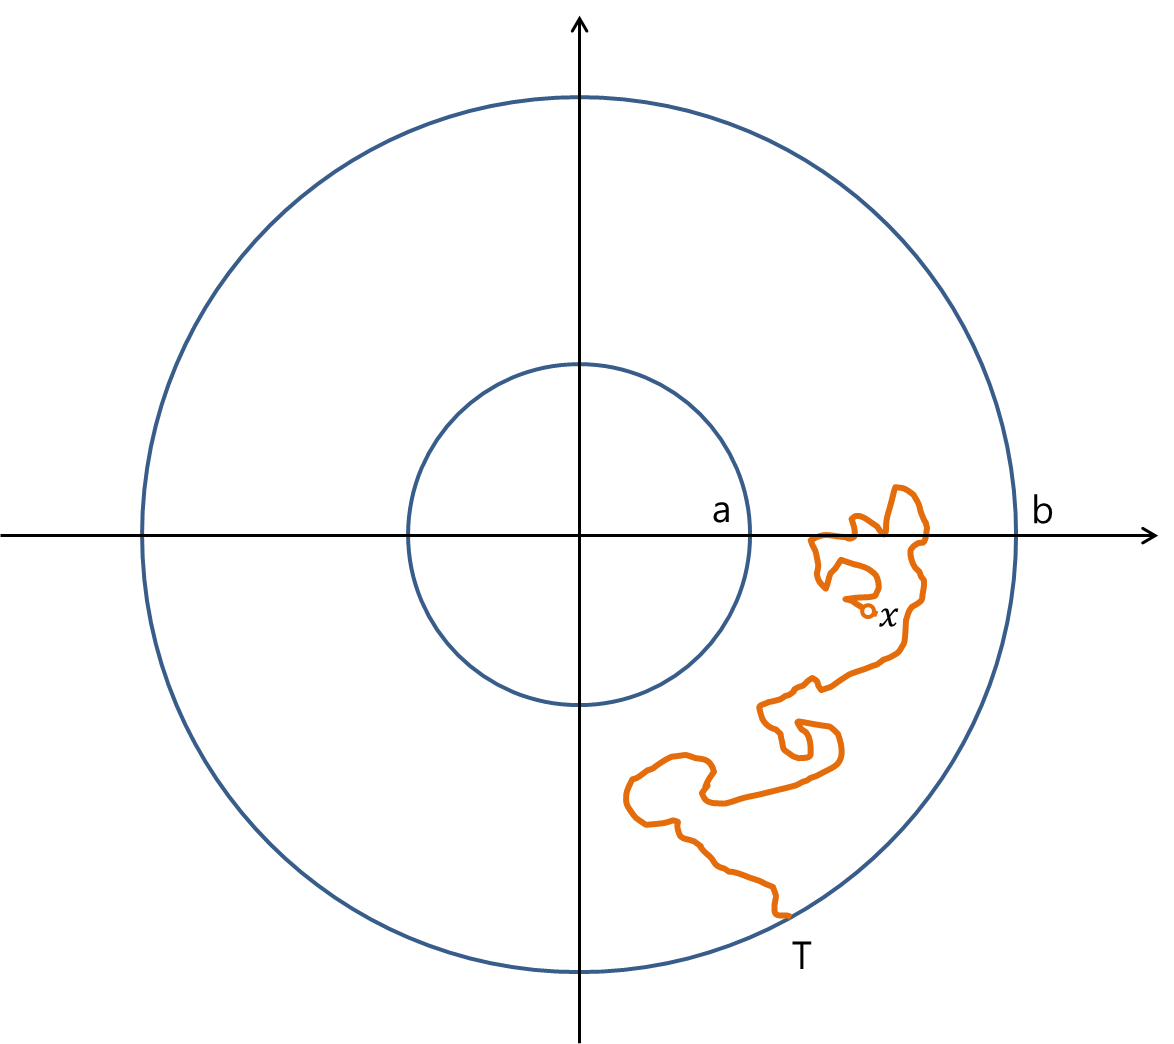
\includegraphics[width=0.33\textwidth]{2}
\end{figure}
Note that $\prob (T< \infty ) =1$. Also for $t\leq T$, $M_t = \log |X_t|$ so $M$ is bounded up to $T$. So optional stopping theorem applies to show
\begin{align*}
0 = \avg (M_0) = \avg(M_T) = \avg( \log |X_t|) = p\log a + (1-b) \log b
\end{align*}
where $p = p(a,b) =\prob (|X_T| =a)$. Consider the limit $a\rightarrow 0$, then $\log a \rightarrow -\infty$, so $p\rightarrow 0$. Hence for $|x|=1$, $p_0(x) = \lim_{b\rightarrow \infty} \lim_{a\rightarrow 0} p(a,b) =0$. By scaling, we see $p_0(x) =0$ for all $x\neq 0$.

\quad In the case $x=0$, for $n\in \mathbb{N}$, by Markov property,
\begin{align*}
\prob (|X_t| =0 \text{ for some }  t \geq \frac{1}{n}) = \int_{\reals^2} p(\frac{1}{n},0,y) p_0(y) dy =0
\end{align*} 
Let $n\rightarrow \infty$ to see $p_0(0) =0$.
\s

For $|x|=1$, let $b\rightarrow \infty$ with $a= \epsilon$ fixed. Since $\log b \rightarrow \infty$, $p(a,b)  \rightarrow 1$ so
\begin{align*}
p_{\epsilon} (x) = \lim_{b\rightarrow \infty} p(\epsilon, b)=1.
\end{align*}
By scaling $p_{\epsilon}(x) =1$ for all $x\neq 0$.

\quad If $x=0$, for $n\in \mathbb{N}$, by Markov property
\begin{align*}
\prob(|X_t| \leq \epsilon \text{ for some } t\geq n) = \int_{\reals^2} p(n,x,y) p_{\epsilon}(y) dy =1
\end{align*}
Hence $\prob(\{ t\geq 0, |X_t| \leq \epsilon \}$ is unbounded $)=1$.
\item[(c)] It will suffice to consider case $d=3$ and to show for all $N\in \mathbb{N}$ that
\begin{align*}
\prob ( \{ t\geq 0 : |X_t| \leq N  \} \text{ is unbounded} ) =0
\end{align*}
We repeat the argument from (b) with $1/|x|$ in place of $\log (|x|)$ - in $d=3$, $1/|x|$ is the harmonic function on $\reals^3 \backslash \{ 0 \}$ - to obtain
\begin{align*}
\frac{p}{a} + \frac{1-p}{b} =1
\end{align*}
for $p = \prob(|X_T|=a)$ and $(X_T)_{t\geq 0} \sim \text{BM}_x (\reals^3)$, $|x|=1$. Let $b\rightarrow \infty$ to see 
\begin{align*}
\lim_{b\rightarrow \infty} p(a,b)  =\prob (|X_t| \leq a \text{ for some } t\geq 0) =a
\end{align*} 
By scaling, for $|x| = N+1$,
\begin{align*}
\prob( |X_t| \leq N \text{ for some } t\geq 0) = \frac{N}{N+1}
\end{align*}
Set $T_0 =0$ and for $k\geq 1$,
\begin{align*}
S_k = \inf \{ t\geq T_{k-1} : |X_t| = N+1 \}, \quad T_k = \inf \{ t \geq S_k : |X_t| =N \}
\end{align*}

Then
\begin{align*}
\prob( T_k < \infty) \leq \frac{N}{N+1} \prob (T_{k-1} < \infty) \leq \Big(\frac{N}{N+1} \Big)^k \rightarrow 0
\end{align*}
by strong Markov property and induction. Set $K = \sup \{ k : T_k < \infty  \}$. Then $K< \infty$ a.s. Now for all $k \geq 1$, on $\{T_{k-1} < \infty \}$, has $S_{k} < \infty$ a.s. Hence $S_{K+1} < \infty$ a.s. But on $\{S_{K+1} \leq \infty \}$, has $|X_t| >N$ for all $t\geq S_{K+1}$ hence $\prob( \{ t\geq 0 : |X_t | \leq N \}$ is unbounded $)= 0$.
\end{itemize}

\eop
\end{proof}

\subsection*{7.9. Brownian Motion and the Dirichlet Problem}

Let $D$ be a connected open set in $\reals^d$. Write $\partial D$ for the boundary. Let $c: D \rightarrow [0,\infty)$, $f: \partial D \rightarrow [0,\infty)$ be measurable functions. For $x\in \overline{D}$, let $(X_t)_{t\geq 0}$ be a Brownian motion starting at $x$.

\quad Define the \textbf{expected total cost} by
\begin{align*}
\phi(x) = \avg \Big( \int_0^T c(X_t) dt + f(X_T) 1_{t< \infty} \Big)
\end{align*}
where $T = \inf \{ t\geq 0 : X_t \not\in D \}$. By a

\quad By a \textbf{solution of the Dirichlet problem (in $D$ with data $c$ and $f$)}, we mean a function $\psi \in C(\overline{D}) \cap C^2 (D)$ such that
\begin{align*}
\begin{cases}
\begin{array}{ll}
-\frac{1}{2} \Delta \psi = c & \text{in } D \\
\psi = f & \text{on } \partial D
\end{array}
\end{cases}
\end{align*}
Accordingly, say $\psi$ is a \textbf{super-solution} if $-\frac{1}{2} \Delta \psi \geq c$, $\psi \geq f$, and call $\psi$ a \textbf{sub-solution} with inverse inequalities.

\quad Suppose $\psi \in C_b^2(\reals^d)$ restrict to a solution of Dirichlet problem on $D$. Consider the martingale (as in \textbf{Theorem 7.5.1})
\begin{align*}
M_t = \psi(X_t) - \psi(X_0) - \int_0^t \frac{1}{2} \Delta \psi (X_s) ds
\end{align*}
Suppose we could justify optional stopping theorem at $T$ and suppose $T< \infty $ a.s. Then
\begin{align*}
0 = \avg(M_0) = \avg(M_T) = \avg(\phi(X_T)) - \psi(x) - \avg(\int_0^T \frac{1}{2} \Delta \psi(X_s) ds)
\end{align*} 
so 
\begin{align*}
\psi(x) = \avg(f(X_T)) + \avg(\int_0^T c(X_s) ds) = \phi(x)
\end{align*}
We will spend time in exploring the condition in which this holds.
\s

\newday

(19th November, Monday)
\s

Settings from the last lecture : $D$ a connected open set $\subset \reals^d$, $c: D \rightarrow [0,\infty)$, $f: \partial D \rightarrow [0,\infty)$ measurable functions,
\begin{align*}
\phi(x) = \avg\Big[ \int_0^T c(X_t) dt + f(X_T) 1_{T<\infty} \Big]
\end{align*}
$(X_t)_{t\geq 0} \sim \text{BM}_x(\reals^d)$, $T= \inf \{ t\geq 0 : X_t \not\in D \}$, times spent in $B\subset D$ before leaving.
\s

\thmnum{7.9.2 (a)} Let $\psi$ be a \emph{non-negative super-solution} of the Dirichlet Problem(DP), $\psi \in C(\overline{D}) \cap C^2(D)$,
\begin{align*}
\begin{cases}
\begin{array}{ll}
-\frac{1}{2} \Delta \psi \geq c & \text{in } D \\
\psi \geq f & \text{on } \partial D
\end{array}
\end{cases}
\end{align*}
Then $\psi \geq \phi$.
\begin{proof}
\pf Clear that $\psi \geq \phi$ on $\partial D$. Fix $x\in D$ and $N\geq 1$ such that $x\in D_N = \{ y\in D : |y|<N, \text{dist}(y,\partial D) > 1/N \}$. There exists $g\in C_b^2(\reals^d)$ such that $g= \psi$ on $D_N$. Consider
\begin{align*}
M_t = g(X_t) - g(X_0) - \int_0^t \frac{1}{2} \Delta g(X_s) ds
\end{align*}
and $T_N =\inf \{ t\geq 0 : X_t \not\in D_N \}$. Then $M$ is a martingale. By the optional stopping theorem, has
\begin{align*}
0 = \avg(M_0) = \avg(M_{T_N \wedge t} ) = \avg(\psi(X_{T_N \wedge t})) - \psi(x) + \avg \Big[ \int_0^{T_N \wedge t} \Big(-\frac{1}{2} \Delta \psi \Big) (X_s) ds \Big]  \quad \cdots \cdots\cdots (\star)
\end{align*}
Consider the limit $N\rightarrow \infty$ and then $t\rightarrow \infty$. Then $T_N \wedge t \nearrow T$, hence
\begin{align*}
\avg \int_0^{T_N \wedge t} \Big(-\frac{1}{2} \Delta \psi \Big) (X_s) ds \geq \avg \int_0^{T_N \wedge t} c(X_s) ds \rightarrow \avg \int_0^T c(X_s) ds
\end{align*}
by monotone convergence. On $\{T < \infty \}$,
\begin{align*}
\psi( X_{T_N \wedge t}) \rightarrow \psi(X_T) \quad \text{a.s.}
\end{align*}
so sine $\psi \geq 0$, by Fatou's lemma,
\begin{align*}
\liminf \avg( \psi(X_{T_N \wedge t})) \geq \avg(\psi(X_T) 1_{T<\infty}) \geq \avg(f(X_T) 1_{T<\infty})
\end{align*}
So taking $\liminf$ in ($\star$), we see $\psi \geq \phi$.

\eop
\end{proof}
\s

\thmnum{7.9.2 (b)} Let $\psi$ be a \emph{non-negative bounded solution} of the Dirichlet Problem, $\psi \in C(\overline{D}) \cap C^2(D)$
\begin{align*}
\begin{cases}
\begin{array}{ll}
-\frac{1}{2} \Delta \psi = c & \text{in } D \\
\psi = f & \text{on } \partial D
\end{array}
\end{cases}
\end{align*}
and suppose that $\avg(\psi(X_t)1_{t<T}) \rightarrow 0$ as $t\rightarrow \infty$($\cdots (\dagger$)). Then $\psi = \phi$.

\textbf{Remark about the condition ($\dagger$) :} Since we assume $\psi$ bounded and
\begin{align*}
|\avg(\psi | X_t) 1_{t<T}| \leq \norms{\psi}{\infty} \prob(t< T)
\end{align*}
We see condition ($\dagger$) holds whenever $T< \infty$ a.s. for all starting points $x$. e.g. we're OK if ($d=1$ and $\partial D \neq \varnothing$) or ($d=2$ and $\reals^2 \backslash D$ contains an open ball) or ($d\geq 3$ and $D$ bounded).
\begin{proof}
\pf Clear that $\psi = \phi$ on $\partial D$. Fix $x\in D$ and $N\geq 1$ such that $x\in D_N = \{ y\in D : |y|<N, \text{dist}(y,\partial D) > 1/N \}$. There exists $g\in C_b^2(\reals^d)$ such that $g= \psi$ on $D_N$. Consider
\begin{align*}
M_t = g(X_t) - g(X_0) - \int_0^t \frac{1}{2} \Delta g(X_s) ds
\end{align*}
and $T_N =\inf \{ t\geq 0 : X_t \not\in D_N \}$. Then $M$ is a martingale. By the optional stopping theorem, has
\begin{align*}
0 = \avg(M_0) = \avg(M_{T_N \wedge t} ) = \avg(\psi(X_{T_N \wedge t})) - \psi(x) + \avg \Big[ \int_0^{T_N \wedge t} \Big(-\frac{1}{2} \Delta \psi \Big) (X_s) ds \Big]  \quad \cdots \cdots\cdots (\star)
\end{align*}
Consider the limit $N\rightarrow \infty$ and then $t\rightarrow \infty$. Then $T_N \wedge t \nearrow T$, hence
\begin{align*}
\avg \int_0^{T_N \wedge t} \Big(-\frac{1}{2} \Delta \psi\Big) (X_s) ds = \avg \int_0^{T_N \wedge t} c(X_s) ds \rightarrow \avg \int_0^T c(X_s) ds
\end{align*}
by monotone convergence. Now 
\begin{align*}
\avg(\psi (X_{T_N \wedge t})) = \avg( \psi(X_{T_N}) 1_{T_N \leq t} ) + \avg(\psi(X_t) 1_{t< T_N})
\end{align*}
We have, sine $\psi \in C(\overline{D})$,
\begin{align*}
\psi(X_{T_N}) 1_{T_N \leq t} \rightarrow \psi(X_T) 1_{T< \infty} \quad \text{a.s.}
\end{align*}
and since $\psi$ is bounded, by dominated convergence,
\begin{align*}
\avg \Big[ \psi(X_{T_N}) 1_{T_N \leq t} \Big] \rightarrow \avg (\psi(X_T) 1_{T<\infty}) = \avg (f(X_T) 1_{T<\infty})
\end{align*}
Also by the assumption
\begin{align*}
\lim_{N\rightarrow \infty} \avg (\psi(X_t) 1_{t< T_N}) = \avg(\psi(X_t) 1_{t<T}) \rightarrow 0 \quad \text{as } t\rightarrow \infty
\end{align*}
Take limit in ($\star$) to see $\psi = \phi$.
\eop
\end{proof}
\s

This theorem tells us about uniqueness of solution of the Dirichlet problem, but it does not say anything about existence of the solution. We are next going to examine this problem.
\s

\thmnum{7.9.2 (c).(I)} Assume $d\geq 3$ and $D= \reals^d$ and $c$ has compact support and $c\in C^2(D)$. Then $\phi \in C^2(\reals^d)$ and $-\frac{1}{2} \Delta \phi =c$.
\begin{proof}
\pf Suppose $g$ is continuous and of compact support on $\reals^d$. Note
\begin{align*}
P_t g(x) = \avg g(x+X_t) = \int_{\reals^d} (2\pi t)^{-d/2} e^{-|x-y|^2/2t} g(y) dy
\end{align*}
where $(X_t)_{t\geq 0} \sim \text{BM}(\reals^d)$ so 
\begin{align*}
\begin{cases}
\norms{P_t g}{\infty}  \leq \norms{g}{\infty} \quad \text{\emph{and also}} \\
\norms{P_t g}{\infty} \leq (2\pi t)^{-d/2} \text{vol}(\text{supp}(g)) \norms{g}{\infty}
\end{cases} \quad \cdots \cdots\cdots (\diamond)
\end{align*}
So splitting the integral at 1 gives
\begin{align*}
\avg \int_0^t g(x+X_t) dt = \int_0^{\infty} P_t g(x) dt \leq (1+ \text{vol}(\text{supp}(g))) \norms{g}{\infty}
\end{align*}
Hence also for $\epsilon >0$,
\begin{align*}
\avg \int_0^{\infty} \sup_{|x-y|< \epsilon} |g(y+X_t)| dt < \infty
\end{align*}
(note, $g_{\epsilon}(x) = \sup_{|y-x| < \epsilon } |g(y)|$ is also continuous of compact support.) Now we can apply this to and its derivative to justify differentiating
\begin{align*}
\phi(x) = \avg \int_0^{\infty} c(x+X_t) dt
\end{align*}
under the integrals to obtain $\phi \in C^2(D)$ and 
\begin{align*}
\Delta  \phi(x) = \avg \int_0^{\infty} \Delta c(x+X_t) dt = \Big( \int_0^s + \int_s^t + \int_t^{\infty} \Big) \avg(\Delta c(x+X_r)) dr
\end{align*} 
for $0<s<t$. Consider the limits $s\rightarrow 0$ and $t\rightarrow \infty$. First and the third integrals tend to 0 using the estimates above. Now
\begin{align*}
\frac{1}{2} \int_s^t  \avg(\Delta c(x+X_r)) dr &= \frac{1}{2} \int_s^t \int_{\reals^d} \Delta c(y) p(r,x,y) dydr \\
&= \frac{1}{2} \int_s^t \int_{\reals^d} c(y) \Delta p(t,x,y) dy dr \\
& = \int_s^t \int_{\reals^d} c(y) \dot{p} (r,x,y) dydr \\
&= \int_{\reals^d} c(y) (p(t,x,y)-p(s,x,y)) dy \quad (\text{FTC})
\end{align*}
But $\int c(y) p(t,x,y) dy \rightarrow 0$ as $t\rightarrow \infty$ and $\int c(y)p(s,x,y) dy = \avg (c(x+X_s)) \rightarrow c(x)$ as $s\rightarrow 0$. Hence $-\frac{1}{2} \Delta \psi =c$ as required.

\eop 
\end{proof}
\s

\newday

(21st November, Wednesday)
\s

(part iii drop-in hours tomorrow 10:30 - 12:30).

(Bring a few different colored pens to class on Friday, if possible)

(Office hours on Monday, time and place TBD)
\s

\thmnum{7.9.4} Let $D$ be a connected open set $\subset \reals^d$ and let $\phi$ be a \emph{non-negative} measurable function on $D$. Suppose
\begin{align*}
\phi(x) = \int_{S(x,p)} \phi(y) \sigma_{x,p}(dy)
\end{align*}
whenever $B(x,p) \subset D$ where $\sigma_{x,p}$ is the uniform distribution on $S(x,p) = \{ y : |x-y| =p \}$. Then \emph{either} $\phi(x) = \infty$ for all $x$ \emph{or} $\phi \in C^{\infty}(D)$ with $\Delta \phi =0$.
\s

This would not be examinable, and will not be proved in the lecture - see online notes for proof.
\s

\thmnum{7.9.5} \emph{(Blumenthal's zero-one law)} Let $(X_t)_{t\geq 0} \sim \text{BM}_x(\reals^d)$. Then for all $A\in \F_{0+}^{X} = \bigcap_{t>0} \F_{t}^X$, has $\prob(A) \in \{ 0,1\}$.
\begin{proof}
\pf Consider the $\pi$-system $\mathscr{A} = \bigcup_{s>0} \sigma (X_t - X_s : t\geq s)$. Then for all $A_0 \in \F_{0+}^X$ and all $A \in \mathscr{A}$, we have $\prob(A_0 \cap A) = \prob(A_0) \prob(A)$. By Dynkin's lemma, this extend to all $A\in \sigma(\mathscr{A})$ (check details).

Now for all $s>0, t\geq s$, $X_t - X_s$ is $\sigma(\mathscr{A})$-measurable. But $X_s \rightarrow 0$ as $s\rightarrow 0$, so $X_t$ is $\sigma(\mathscr{A})$-measurable. So $\F_{\infty}^X = \sigma(\mathscr{A}) \supset \F_{0+}^X$. So for $A\in \F_{0+}^X$,
\begin{align*}
\prob(A) = \prob(A\cap A) = \prob(A)\prob(A)
\end{align*}
and therefore $\prob(A) \in \{0,1\}$.

\eop
\end{proof}
\s

\propnum{7.9.6} \emph{(Brownina motion enters all cones immediately)} Let $A$ be an open subset of $S^{d-1}$ and let $\epsilon>0$. Set $C$ a cone,
\begin{align*}
C = \{ty : y\in A, t\in (0,\epsilon) \}
\end{align*} 
Let $X \sim \text{BM}_0(\reals^d)$, and define $T_C = \inf \{ t\geq 0: X_t \in T_C \}$. Then $\prob(T_C =0)=1$. 
\begin{proof}
See example sheet.
\end{proof}
\s

Some definition (\textbf{External cone condition, ECC))} : Let $D \subset \reals^d$ be open and connected. Then $D$ satisfies ECC if for all $x\in \partial D$ , there exist $A$ open $\subset S^{d-1}$, $\epsilon >0$ such that
\begin{align*}
\{x+ty : t\in (0,\epsilon), y\in A \} \cap D = \phi
\end{align*}
This is weaker than the Lipschitz boundary condition.

\s
\thmnum{7.9.2(c)} Let $D$ be a connected open set $\subset \reals^d$. Let $c\in C^2(\reals^d)$, $f\in C(\partial D)$. Set
\begin{align*}
\phi(x) = \avg \Big( \int_0^T c(X_t) dt + f(X_T) 1_{T<\infty} \Big) \quad \forall x\in \overline{D}
\end{align*}
where $X \sim \text{BM}_0(\reals^d)$ and $T = \inf \{ t\geq 0: X_t \not\in D \}$. Assume $D$ satisfies the \emph{external cone condition(ECC)} and that $\phi$ is locally bounded. Then $\phi \in C^2(D) \cap C(\overline{D})$ and $-\frac{1}{2}\Delta \phi =c$ in $D$ and $\phi =f$ on $\partial D$. i.e. $\phi$ solves the Dirichlet condition.
\s

This is significant - the proof using ECC is hard to achieve just using usual theories of partial differential equations.(recall, we usually prove theorems under Lipschitz boundary condition in PDEs). Probability wins!
\s

\lemnum{7.9.3} Let $D_0$ be a \emph{bounded subset} of $D$. Define $T_0 = \inf \{t\geq 0: X_t \not\in D_0 \}$, $x\in \overline{D}$. Then
\begin{align*}
\phi(x) = \avg \Big( \int_0^{T_0} c(X_t) dt + \phi(X_{T_{0}}) \Big)
\end{align*}
\begin{proof}
\pf Set $\tilde{X}_t = X_{T_0 +t}$, $\tilde{\F}_{t} = \F_{T_0 +t}$, and $\tilde{T} = \inf \{ t\geq 0 : \tilde{X}_t \not\in D \}$. By \emph{Strong Markov property}, $(\tilde{X}_t)$ is an $(\tilde{\F}_t)$-BM. Now
\begin{align*}
\int_0^T c(X_t) dt + f(X_T) 1_{T<\infty} = \int_0^{T_0} c(X_t) dt + \int_0^{\tilde{T}} c(X_t) dt + f(\tilde{X}_{\tilde{T}})1_{\tilde{T}<\infty} \quad \cdots\cdots\cdots (\dagger)
\end{align*}
Here we used that $\tilde{T}<\infty$ \emph{iff} $T<\infty$ and $X_T = \tilde{X}_{\tilde{T}}$. By \textbf{Prop 7.4.1},
\begin{align*}
\avg( \int_0^{\tilde{T}} c(X_t) dt + f(\tilde{X}_{\tilde{T}})1_{\tilde{T}<\infty} | \F_{T_0} ) = \phi(X_{T_0}) \quad \text{a.s.}
\end{align*}
So we obtain result on taking $\avg$ in ($\dagger$)

\eop
\end{proof}
\s

Recall, we proved \textbf{Theorem 7.9.2(c)} in a weaker setting earlier. Here, we prove in a slightly more general setting.
\begin{proof}
\textbf{proof of Theorem 7.9.2(c) II.} We show in the case $c=0$ that $\phi \in C^{\infty}(D)$ with $\Delta \phi =0$ -then follows from a simple argument using symmetry of a sphere and \textbf{Theorem 7.9.4}.

See online notes.
\end{proof}
\s

\begin{proof}
\textbf{proof of Theorem 7.9.2(c) III.} We show for all $y \in \partial D$ that
\begin{align*}
\lim_{x\rightarrow y, x\in \overline{D}} \phi(x) = \phi(y)
\end{align*}
Fix $y\in \partial D$ and choose $U$ bounded open set $\subset \reals^d$ with $u\in U$. Set $D_0 = D \cap U$. By \emph{exterior cone condition}, there exist $A\in S^{d-1}$, $\epsilon>0$ such that $\{y+tz : t \in (0,\epsilon) , z\in A \} \cap D = \phi$. Let $(X_t)_{t\geq 0}$ be a $\text{BM}_0(\reals^d)$. Set $T_0(x) = \inf \{ t\geq 0: x+ X_t \not\in D \}$. By \textbf{Proposition 7.9.6}, for $T_C = \inf \{t\geq 0 : y+X_t \in C \}$ we have $T_C =0$ a.s. Now on the event $\{ T_C =0 \}$, we have $T_0(x) \rightarrow 0$ as $x\rightarrow y$($x$ staying in $\overline{D}$) so $X_{T_0(x)} + x \in \partial D$ eventually as $x\rightarrow y$ and $X_{T_0(x)} +x \rightarrow y$ as $x\rightarrow y$. Hence
\begin{align*}
\phi(X_{T_0(x)} +x) = f(X_{T_0(x)} +x) \rightarrow f(y) \quad \text{as }x\rightarrow y
\end{align*}
Also by \textbf{Prop 7.7.1}, $\avg(\sup_{x\in D_0} T_0(x)) < \infty$. Now
\begin{align*}
\phi(x) = \avg \Big( \int_0^{T_0(x)} c(x+X_t)dt + \phi(X_{T_0(x)} + x) \Big)
\end{align*}
Let $x\rightarrow y$, then using dominated convergence to see $\phi(x) \rightarrow f(y)$ as $x\rightarrow y$.

\eop
\end{proof}
\s

\newday

(23rd November, Friday)
\s

The following is the last part of proof of \textbf{Theorem 7.9.2(c)}
\s

\begin{proof}
\textbf{\textbf{proof of Theorem 7.9.2(c) IV.}} It will suffice to consider the case where $d\geq 3$, or set $\tilde{D} = D \times \reals^2$ and extend $c$ as a constant in new directions. 

\quad Consider for now the case $D$ bounded. There exists $\tilde{c} \in C^2(\reals^d)$ of compact support with $\tilde{c} = c$ in $D$. Set
\begin{align*}
\phi_0(x) = \avg \int_0^{\infty} \tilde{c}(X_t) dt
\end{align*}
By \textbf{part I}, $\phi_0 \in C^2(\reals^d)$ with $-\frac{1}{2}\Delta \phi_0 = \tilde{c}$. Now
\begin{align*}
\phi_0(x) = \avg \Big( \int_0^T \tilde{c}(X_t) dt + \phi_0(X_T) \Big) = \phi(x) + \phi_1(x)
\end{align*}
(by \textbf{Lemma 7.9.3}) where $\phi_1(x)  = \avg(\phi_0(X_T))$. By \textbf{part II}, $\phi_1 \in C^{\infty}(D)$ and $\Delta \phi_1 =0$. So $\phi \in C^2 (D)$ and $-\frac{1}{2} \Delta \phi =c$.

\quad Turn to the case $D$ unbounded. Choose any bounded open $D_0 \subset D$. Then
\begin{align*}
\phi (x) = \phi_0(x) + \phi_1(x)
\end{align*}
(new $\phi_0$ and $\phi_1$) where $\phi_0$ and $\phi_1$ are defined by
\begin{align*}
\phi_0(x) = \avg \Big( \int_0^{T_0} c(X_t) dt \Big), \quad \phi_1(x) = \avg(\phi(X_{T_0}))
\end{align*}
where $T_0  = \inf \{ t\geq 0 : X_t \not\in D_0 \}$. We know $\phi_0 \in C^2(D)$ and $-\frac{1}{2}\Delta \phi_0 = c$ and since $\phi$ is locally bounded, $\phi_1 \in C^{\infty}(D_0)$ with $\Delta \phi_1 =0$. Hence $\phi \in C^2(D_0)$ and $-\frac{1}{2}\Delta \phi =c$.

\eop
\end{proof}
\s

Plan for the rest of the course : we will not cover all the materials(e.g. Donsker's invariance principle or Skorohod embedding for random walks) - do not have enough time. But will discuss about Poisson random measures.

\section*{8. Poisson Random Measures}

Our ambition is to classify all stationary independent increments - this is what L\'{e}vy-Khinchin theorem tells us. To prove this, we need some works on Poisson random measures.

\subsection*{8.1. Construction}

For $\lambda \in (0,\infty)$, a random variable $X$ with values in $\mathbb{Z}^+ \cup \{\infty \}$ has distribution $P(\lambda)$ if
\begin{align*}
\prob(X = x) = e^{-\lambda} \frac{\lambda^x}{x!}, \quad x\in \mathbb{Z}^+
\end{align*}
Also conventionally write $X \sim P(0)$ if $X \equiv 0$, and $P \sim P(\infty) $ if $X \equiv \infty$.
\s

\propnum{8.1.1.}\emph{(Addition property)} Let $(N_k : k\in \mathbb{N})$ be a sequence of independent random variables with $N_k \sim P(\lambda_k)$ for all $k$. Then 
\begin{align*}
\sum_{k} N_k \sim P \big( \sum_k \lambda_k \big)
\end{align*}
\s

\propnum{8.1.2.}\emph{(Splitting property)} Suppose $N\sim P(\lambda)$. Let $(Y_n : n\in \mathbb{N})$ be a sequence of i.i.d. random variables in $\mathbb{N}$. Set $N_k = \sum_{n=1}^N 1_{Y_n =k}$ for $k\geq 1$. Then $(N_k : k\in \mathbb{N})$ is a sequence of independent $P(\lambda_k)$ random variables with $\lambda_k = \lambda \prob(Y_1) =k$.
\s

The proofs are just elementary calculations, but please do them!!!
\s

Let $(E, \mathscr{E}, \mu)$ be a \emph{$\sigma$-finite} measure space.

\begin{itemize}
\item A \textbf{Poisson random measure} of intensity $\mu$ is a map $M : \Omega \times \mathscr{E} \rightarrow \mathbb{Z}^+ \cup \{\infty \}$ (for $A \in \mathscr{E}$, think of $M(A)$ as $M(\{\omega \} \times A)$, a random variable) such that for any disjoint sequence $(A_k : k\in \mathbb{N})$ in $\mathscr{E}$,
\begin{itemize}
\item[(i)] $M(\cup_k A_k) = \sum_k M(A_k)$. 
\item[(ii)] $M(A_k)$ is a $P(\mu(A_k))$ random variable for all $k$.
\item[(iii)] The random variables $M(A_k)$, $k\in \mathbb{N}$ are independent.
\end{itemize}
\item We can construct a $\text{PRM}(\mu)$ as follows.

\quad First in case $\mu(E) < \infty$, take $N\sim P(\lambda)$, $\lambda = \mu(E)$ and take independent random variables $(Y_n : n\in \mathbb{N})$ independent of $N$ with distribution $\frac{1}{\lambda} \mu$. Define $M(A) = \sum_{n=1}^{N} 1_{Y_n \in A}$ Then $M \sim \text{PRM}(\mu)$, i.e. $M(A) \sim P(\mu(A))$. (\textbf{an exercise})

\quad In general, if $\mu(E) = \infty$, as $E$ is $\sigma$-finite, there exist disjoint $E_n \in \mathscr{E}$ with $\cup_{n} E_{n} = E$ such that $\mu(E_n) < \infty$ for all $n$. Using preceding construction, we obtain $(M_n)_n$ independent $\text{PRM}(\mu 1_{E_n})$'s. Then set $M = \sum_n M_n$. Then $M \sim \text{PRM}(\mu)$. (\textbf{also an exercise})

\item The uniqueness of such map also can be shown - refer to the online lecture notes.
\end{itemize}

\subsection*{8.2. Integrals with respect to Poisson Random Measures}

\thmnum{8.2.1} Let $M$ be a $\text{PRM}(\mu)$ and let $g$ be a measurable function on $(E, \mathscr{E})$. Assume $\mu(E) < \infty$. Define
\begin{align*}
M(g) = \begin{cases}
\begin{array}{ll}
\int_E g(y) M(dy) & \text{if  } M(E) < \infty \\
0 & \text{o/w}
\end{array}
\end{cases}
\end{align*}
Then $M(g)$ is a well-defined random variable and 
\begin{align*}
\avg(e^{inM(g)}) = \exp \Big[ \int_E (e^{ing(y)} -1) \mu(dy) \Big]
\end{align*}
and if $g\in L^1(\mu)$ then $M(g) \in L^1(\prob)$ with $\avg(M(g)) = \mu(g)$ and $\text{Var}(M(g)) = \mu(g^2)$.
\begin{proof}
\pf Let's see these all true in the case $M(A) = \sum_{n=1}^N 1_{Y_n \in A}$. Then $M(g) = \sum_{n=1}^N g(Y_n)$ and this is clearly a well-defined measurable function. We have
\begin{align*}
\avg(e^{in M(g)} | N=n) = \avg( e^{in \sum_{k=1}^n g(Y_k) }) =\prod_{k=1}^n \avg( e^{in  g(Y_k) }) = \Big( \int_E e^{in g(y)} \frac{\mu(dy)}{\lambda} \Big)^n
\end{align*}
So 
\begin{align*}
\avg(e^{in M(g)}) &= \sum_{n=0}^{\infty} e^{-\lambda} \frac{\lambda^n}{n!} \Big( \int_E e^{ing(y)} \frac{\mu(dy)}{\lambda} \Big)^n \\
&= e^{-\lambda} \exp \Big( \int_E e^{ing(y)} \mu(dy) \Big)
\end{align*}
so we obtain the average and variance of $M(g)$ from the moment generating function.

\quad For the general case, since $(E, \mathscr{E},\mu)$ is $\sigma$-finite, let $E = \cup_n E_n$ where $E_n \in \mathscr{E}$, disjoint and $\mu(E_n) < \infty$. Let $M_n$ be the Poisson random measure on each $E_n$. Then $1_{M<\infty} \sum_{n=1}^{\infty} M_{n} \rightarrow M 1_{M<\infty}$ . The statement holds for each $M_n$ by above, so by dominated convergence(dominated by 1),
\begin{align*}
\avg(e^{in M(g)}) &= \sum_{n=0}^{\infty} e^{-\lambda} \frac{\lambda^n}{n!} \Big( \int_E e^{ing(y)} \frac{\mu(dy)}{\lambda} \Big)^n \\
&= e^{-\lambda} \exp \Big( \int_E e^{ing(y)} \mu(dy) \Big)
\end{align*}
also holds.

\eop
\end{proof}















\end{document}



